%Wissenschaftliche Mitarbeiter
%Scientific staff

\section*{Wissenschaftliche Mitarbeiter}

	\begin{tabular}{p{2.1cm}p{6cm}p{2cm}p{6cm}}
	% 1. row
	\parbox[c]{2cm}{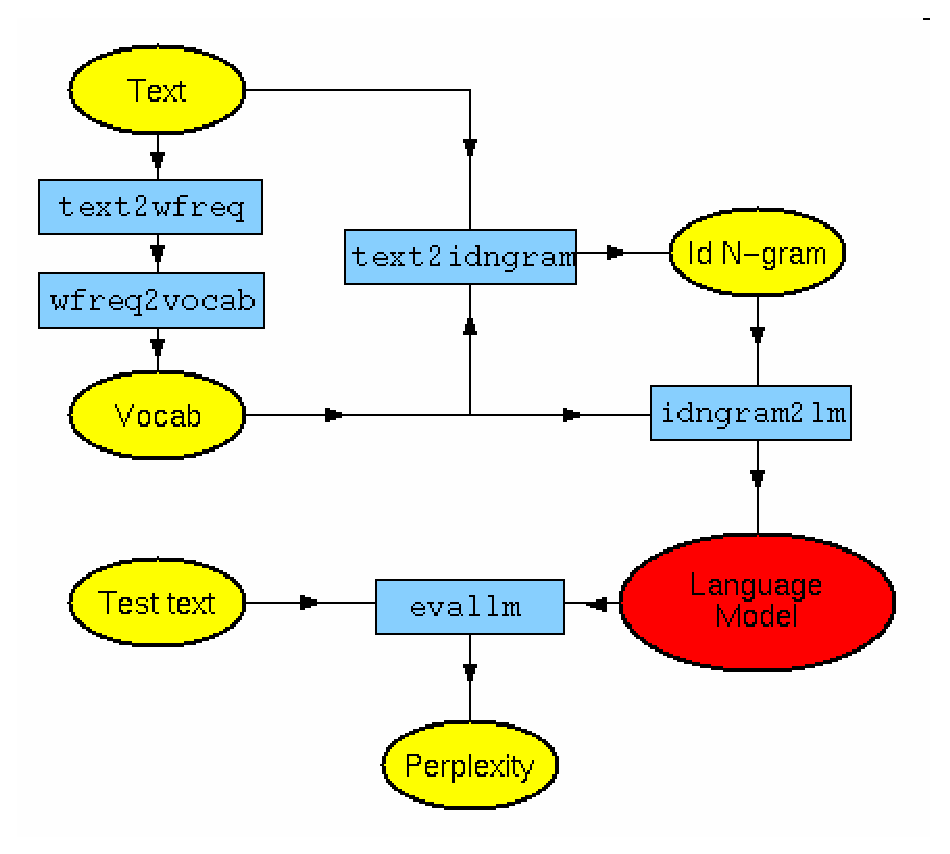
\includegraphics[width=2cm]{Bilder/toolkit.eps}} 	\hfill 	 	
	& \parbox[c]{5.9cm}{
			\Large Dipl.Ing Wilhelm Peters \normalsize \\
			\phantom{test}\\
			Studium der Elektrotechnik\\
			\enfont{Studies in electrical engineering}\\
			Systemoptimierung Fahrantrieb\\
			\enfont{System optimisation traction drive}\\
			\phantom{test}\\
			\phantom{test}\\
		}	
	&	\parbox[c]{2cm}{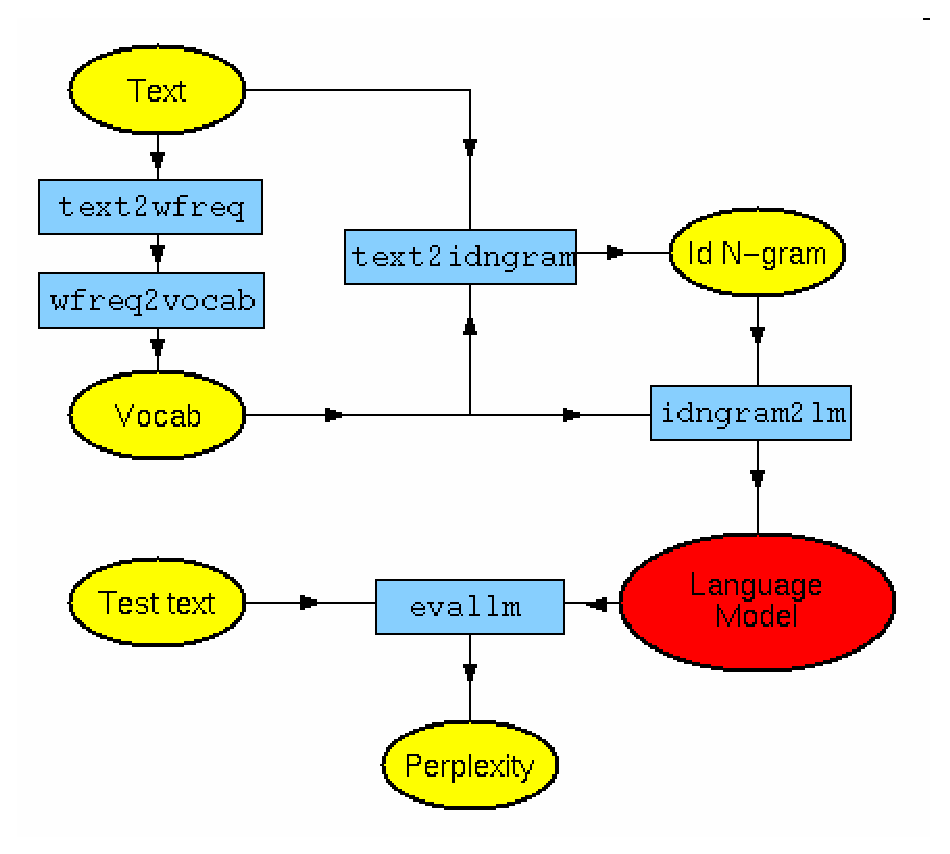
\includegraphics[width=2cm]{Bilder/toolkit.eps}}  	\hfill 		
	
	& \parbox[c]{5.9cm}{
			\Large Dipl.Ing Wilhelm Peters \normalsize \\
			\phantom{test}\\
			Studium der Elektrotechnik\\
			\enfont{Studies in electrical engineering}\\
			Systemoptimierung Fahrantrieb\\
			\enfont{System optimisation traction drive}\\
			Mitarbeiter seit 2007
			\enfont{Member of staff since 2007}\\
		}\\
		%\phantom{Leerzeile} &&&\\
		
	% 2. row
	\parbox[c]{2cm}{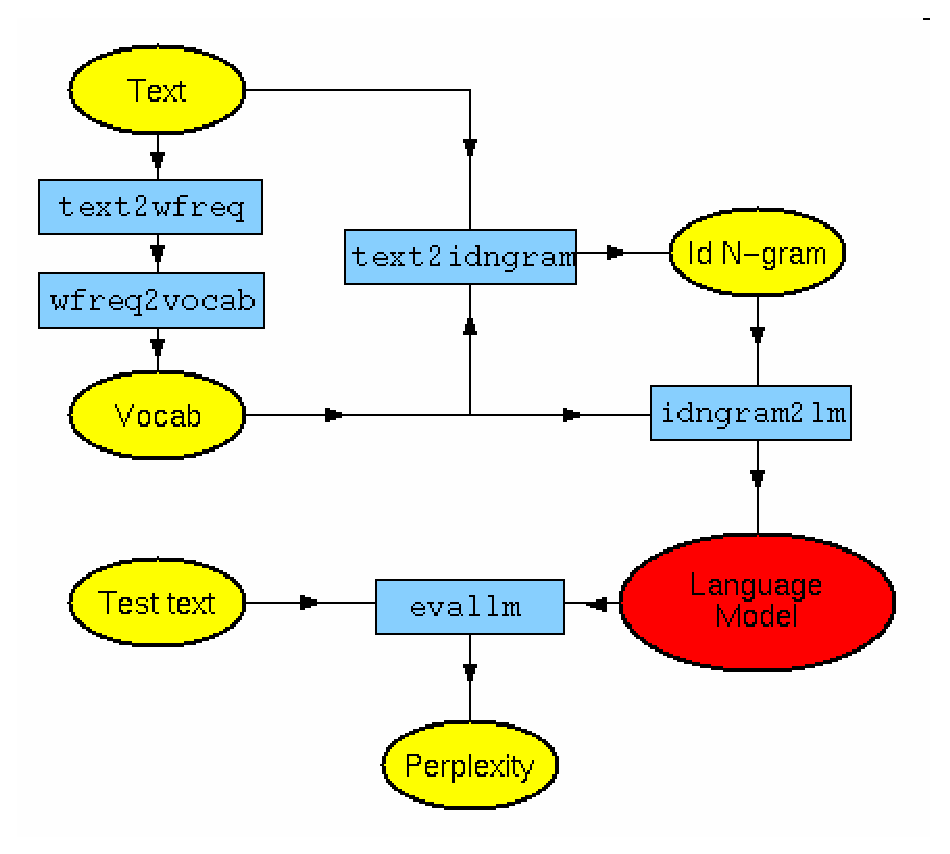
\includegraphics[width=2cm]{Bilder/toolkit.eps}} 	\hfill 	
	& \parbox[c]{5.9cm}{
			\Large Dipl.Ing Wilhelm Peters \normalsize \\
			\phantom{test}\\
			Studium der Elektrotechnik\\
			\enfont{Studies in electrical engineering}\\
			Systemoptimierung Fahrantrieb\\
			\enfont{System optimisation traction drive}\\
			\phantom{test}\\
			\phantom{test}\\
		}	
		
	&	\parbox[c]{2cm}{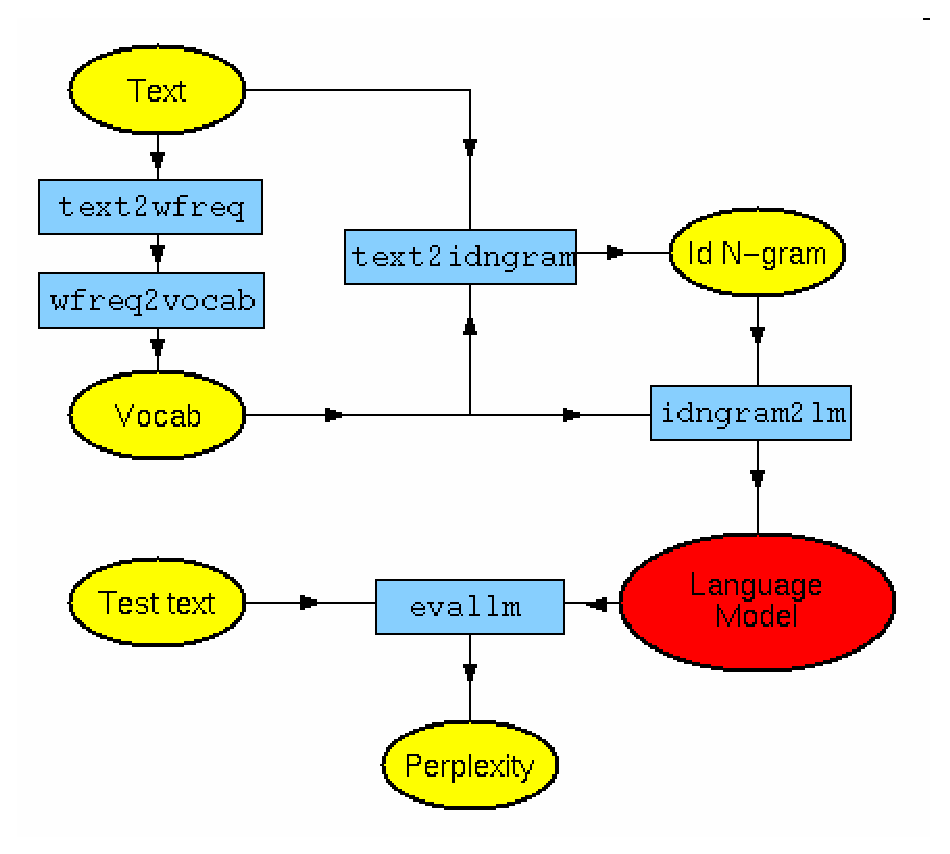
\includegraphics[width=2cm]{Bilder/toolkit.eps}}  	\hfill 	
	& \parbox[c]{5.9cm}{
			\Large Dipl.Ing Wilhelm Peters \normalsize \\
			\phantom{test}\\
			Studium der Elektrotechnik\\
			\enfont{Studies in electrical engineering}\\
			Systemoptimierung Fahrantrieb\\
			\enfont{System optimisation traction drive}\\
			Mitarbeiter seit 2007
			\enfont{Member of staff since 2007}\\
		}\\
	%	\phantom{Leerzeile} &&&\\		
\end{tabular}

Hier ist ein text. \phantom{Und hier ist der Text als phantom}. Hier ist wieder text.